\documentclass[11pt,preprint, authoryear]{elsarticle}

\usepackage{lmodern}
%%%% My spacing
\usepackage{setspace}
\setstretch{1.2}
\DeclareMathSizes{12}{14}{10}{10}

% Wrap around which gives all figures included the [H] command, or places it "here". This can be tedious to code in Rmarkdown.
\usepackage{float}
\let\origfigure\figure
\let\endorigfigure\endfigure
\renewenvironment{figure}[1][2] {
    \expandafter\origfigure\expandafter[H]
} {
    \endorigfigure
}

\let\origtable\table
\let\endorigtable\endtable
\renewenvironment{table}[1][2] {
    \expandafter\origtable\expandafter[H]
} {
    \endorigtable
}


\usepackage{ifxetex,ifluatex}
\usepackage{fixltx2e} % provides \textsubscript
\ifnum 0\ifxetex 1\fi\ifluatex 1\fi=0 % if pdftex
  \usepackage[T1]{fontenc}
  \usepackage[utf8]{inputenc}
\else % if luatex or xelatex
  \ifxetex
    \usepackage{mathspec}
    \usepackage{xltxtra,xunicode}
  \else
    \usepackage{fontspec}
  \fi
  \defaultfontfeatures{Mapping=tex-text,Scale=MatchLowercase}
  \newcommand{\euro}{€}
\fi

\usepackage{amssymb, amsmath, amsthm, amsfonts}

\def\bibsection{\section*{References}} %%% Make "References" appear before bibliography


\usepackage[round]{natbib}

\usepackage{longtable}
\usepackage[margin=2.3cm,bottom=2cm,top=2.5cm, includefoot]{geometry}
\usepackage{fancyhdr}
\usepackage[bottom, hang, flushmargin]{footmisc}
\usepackage{graphicx}
\numberwithin{equation}{section}
\numberwithin{figure}{section}
\numberwithin{table}{section}
\setlength{\parindent}{0cm}
\setlength{\parskip}{1.3ex plus 0.5ex minus 0.3ex}
\usepackage{textcomp}
\renewcommand{\headrulewidth}{0.2pt}
\renewcommand{\footrulewidth}{0.3pt}

\usepackage{array}
\newcolumntype{x}[1]{>{\centering\arraybackslash\hspace{0pt}}p{#1}}

%%%%  Remove the "preprint submitted to" part. Don't worry about this either, it just looks better without it:
\makeatletter
\def\ps@pprintTitle{%
  \let\@oddhead\@empty
  \let\@evenhead\@empty
  \let\@oddfoot\@empty
  \let\@evenfoot\@oddfoot
}
\makeatother

 \def\tightlist{} % This allows for subbullets!

\usepackage{hyperref}
\hypersetup{breaklinks=true,
            bookmarks=true,
            colorlinks=true,
            citecolor=blue,
            urlcolor=blue,
            linkcolor=blue,
            pdfborder={0 0 0}}


% The following packages allow huxtable to work:
\usepackage{siunitx}
\usepackage{multirow}
\usepackage{hhline}
\usepackage{calc}
\usepackage{tabularx}
\usepackage{booktabs}
\usepackage{caption}


\newenvironment{columns}[1][]{}{}

\newenvironment{column}[1]{\begin{minipage}{#1}\ignorespaces}{%
\end{minipage}
\ifhmode\unskip\fi
\aftergroup\useignorespacesandallpars}

\def\useignorespacesandallpars#1\ignorespaces\fi{%
#1\fi\ignorespacesandallpars}

\makeatletter
\def\ignorespacesandallpars{%
  \@ifnextchar\par
    {\expandafter\ignorespacesandallpars\@gobble}%
    {}%
}
\makeatother

\newenvironment{CSLReferences}[2]{%
}

\urlstyle{same}  % don't use monospace font for urls
\setlength{\parindent}{0pt}
\setlength{\parskip}{6pt plus 2pt minus 1pt}
\setlength{\emergencystretch}{3em}  % prevent overfull lines
\setcounter{secnumdepth}{5}

%%% Use protect on footnotes to avoid problems with footnotes in titles
\let\rmarkdownfootnote\footnote%
\def\footnote{\protect\rmarkdownfootnote}
\IfFileExists{upquote.sty}{\usepackage{upquote}}{}

%%% Include extra packages specified by user

%%% Hard setting column skips for reports - this ensures greater consistency and control over the length settings in the document.
%% page layout
%% paragraphs
\setlength{\baselineskip}{12pt plus 0pt minus 0pt}
\setlength{\parskip}{12pt plus 0pt minus 0pt}
\setlength{\parindent}{0pt plus 0pt minus 0pt}
%% floats
\setlength{\floatsep}{12pt plus 0 pt minus 0pt}
\setlength{\textfloatsep}{20pt plus 0pt minus 0pt}
\setlength{\intextsep}{14pt plus 0pt minus 0pt}
\setlength{\dbltextfloatsep}{20pt plus 0pt minus 0pt}
\setlength{\dblfloatsep}{14pt plus 0pt minus 0pt}
%% maths
\setlength{\abovedisplayskip}{12pt plus 0pt minus 0pt}
\setlength{\belowdisplayskip}{12pt plus 0pt minus 0pt}
%% lists
\setlength{\topsep}{10pt plus 0pt minus 0pt}
\setlength{\partopsep}{3pt plus 0pt minus 0pt}
\setlength{\itemsep}{5pt plus 0pt minus 0pt}
\setlength{\labelsep}{8mm plus 0mm minus 0mm}
\setlength{\parsep}{\the\parskip}
\setlength{\listparindent}{\the\parindent}
%% verbatim
\setlength{\fboxsep}{5pt plus 0pt minus 0pt}



\begin{document}



\begin{frontmatter}  %

\title{Question 1: COVID}

% Set to FALSE if wanting to remove title (for submission)




\author[Add1]{Grace Grant}
\ead{21653488@sun.ac.za}





\address[Add1]{Stellenbosch University, Stellenbosch, South Africa}



\vspace{1cm}





\vspace{0.5cm}

\end{frontmatter}

\setcounter{footnote}{0}



%________________________
% Header and Footers
%%%%%%%%%%%%%%%%%%%%%%%%%%%%%%%%%
\pagestyle{fancy}
\chead{}
\rhead{}
\lfoot{}
\rfoot{\footnotesize Page \thepage}
\lhead{}
%\rfoot{\footnotesize Page \thepage } % "e.g. Page 2"
\cfoot{}

%\setlength\headheight{30pt}
%%%%%%%%%%%%%%%%%%%%%%%%%%%%%%%%%
%________________________

\headsep 35pt % So that header does not go over title




\hypertarget{total-deaths-per-continent}{%
\section{Total deaths per continent}\label{total-deaths-per-continent}}

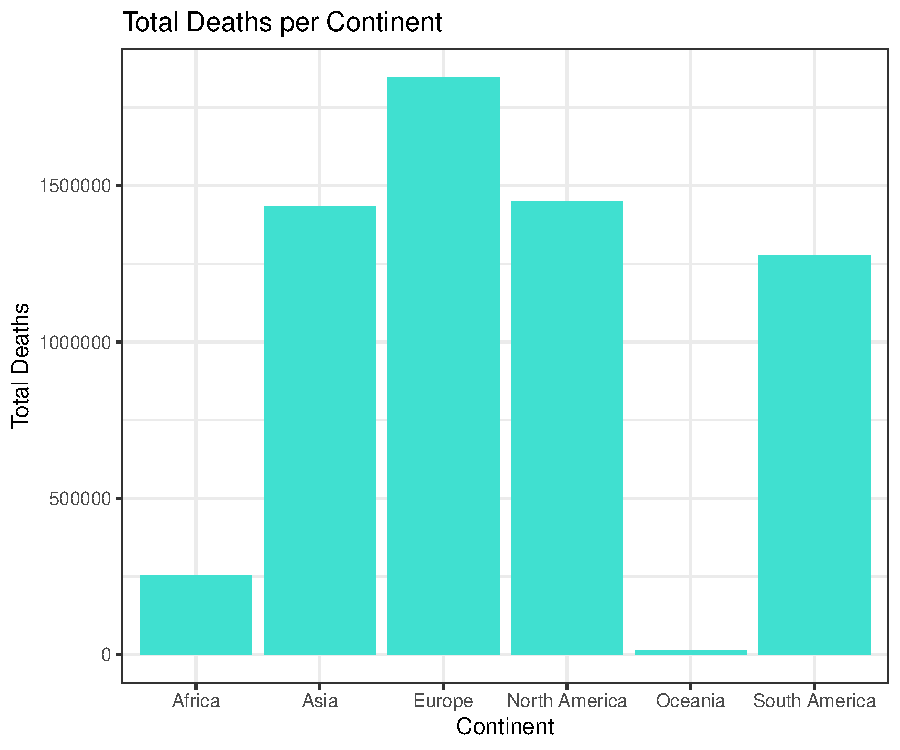
\includegraphics{Question-1_files/figure-latex/unnamed-chunk-1-1.pdf}

We can see from the above graph how each continent was affected by the
pandemic, according to the total number of deaths. Europe, North America
and Asia had the highest number of deaths which could be linked to their
population sizes as well as the proximity in which people live in those
regions. Africa and Oceania had the least deaths which could be a result
of many factors, one of which is a lack of or incorrect reporting of
deaths, especially in Africa.

\hypertarget{trajectory-of-cases-in-2020-per-continent}{%
\section{Trajectory of cases in 2020 per
continent}\label{trajectory-of-cases-in-2020-per-continent}}

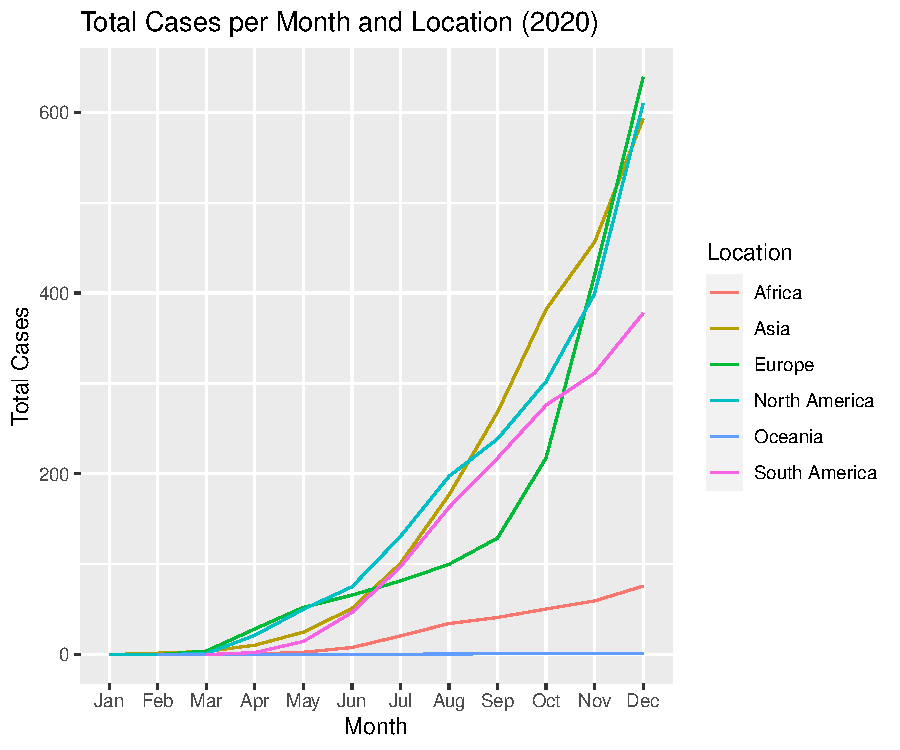
\includegraphics{Question-1_files/figure-latex/unnamed-chunk-2-1.pdf}

This graph provides some insight into how the different continents
experienced the update of COVID cases in 2020 when the pandemic began.
Similar to the previous graph, Africa had a much lower total number of
cases compared to Europe, Asia and North America. It is also interesting
to note that cases only began to pick up in Africa towards the middle of
the year while, for the Northern Hemisphere, cases were already
accumulating from March/April.

\hypertarget{total-deaths-in-different-countries-based-on-population-age-poverty-and-diabetes-prevalence}{%
\section{Total deaths in different countries based on population age,
poverty and diabetes
prevalence}\label{total-deaths-in-different-countries-based-on-population-age-poverty-and-diabetes-prevalence}}

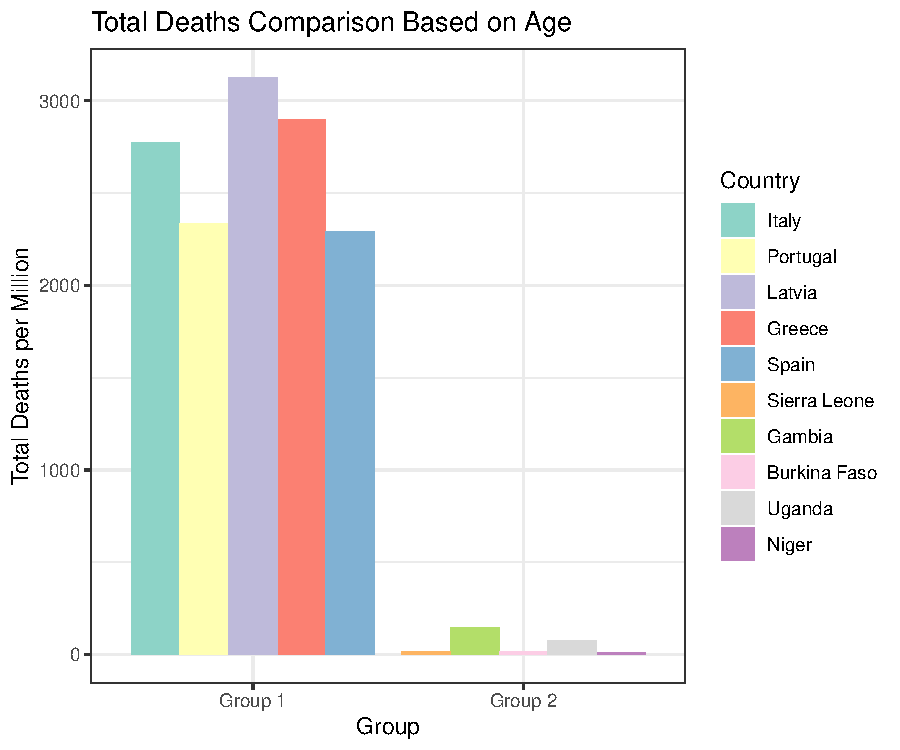
\includegraphics{Question-1_files/figure-latex/unnamed-chunk-3-1.pdf}
\newpage
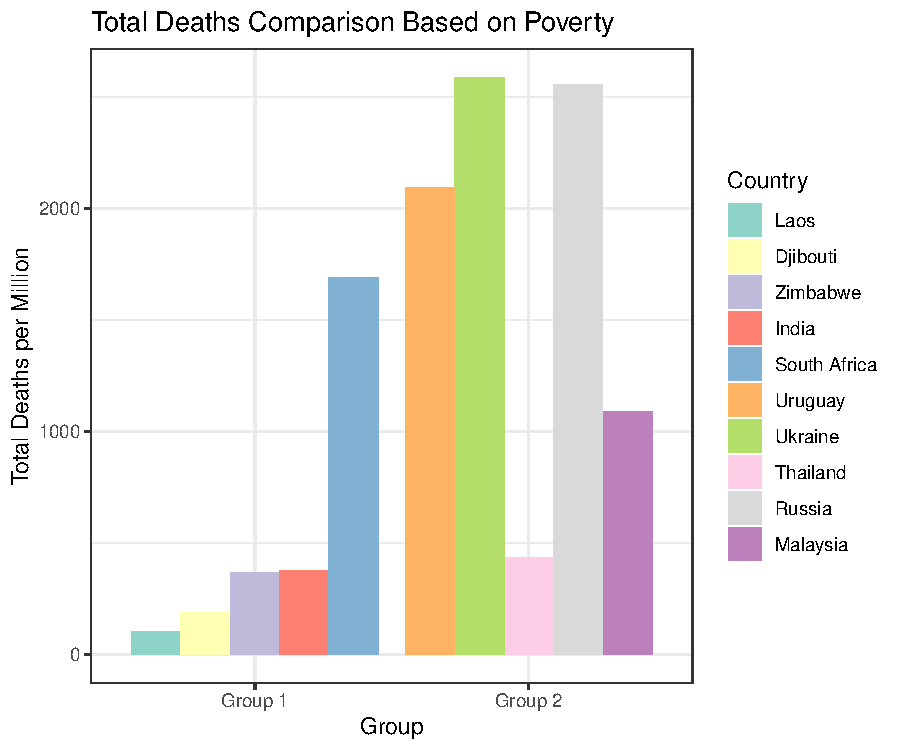
\includegraphics{Question-1_files/figure-latex/unnamed-chunk-4-1.pdf}
\newpage
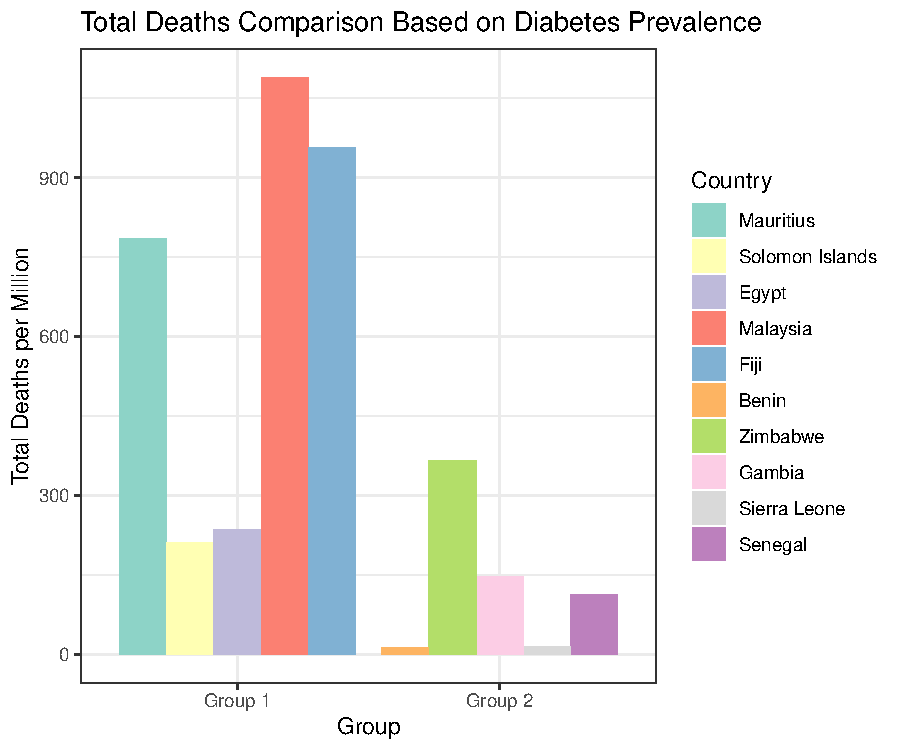
\includegraphics{Question-1_files/figure-latex/unnamed-chunk-5-1.pdf}

The three graphs provided produce some interesting results. Firstly,
countries that had the highest percentage of the population aged older
than 70 experienced much greater deaths than the countries that had
younger populations. This makes sense given that older people are more
susceptible to getting COVID and then dying from it. The third graph
also makes sense, showing that countries with a higher prevalence of
diabetes had more deaths from COVID. However, the second graph is
somewhat counterintuitive in that poorer countries (those with higher
levels of extreme poverty) mostly had fewer deaths than wealthier
countries. Some reasons for this may be that the poor countries are in
Africa which has the fewest deaths or that the metric for poverty
includes so many other factors that it is difficult to establish a
strong correlation between poverty and deaths from COVID.

\hypertarget{weekly-icu-and-hospital-admissions}{%
\section{Weekly ICU and hospital
admissions}\label{weekly-icu-and-hospital-admissions}}

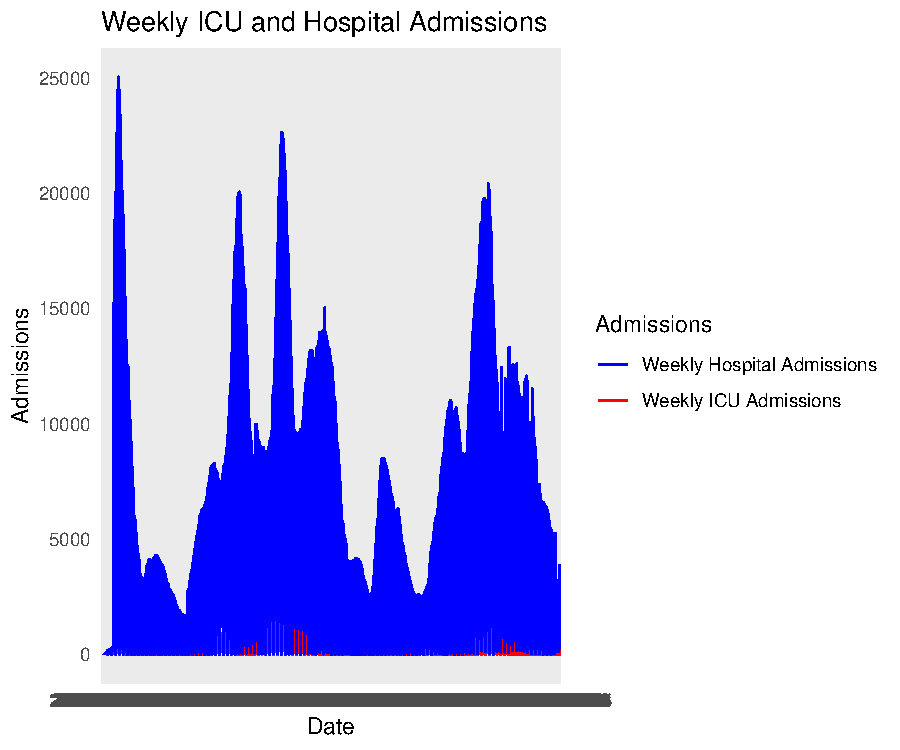
\includegraphics{Question-1_files/figure-latex/unnamed-chunk-6-1.pdf}

It is also interesting to consider hospitalisation figures, which are
shown by weekly ICU and weekly hopsital admissions in the above graph.
It is evident that ICU admissions are much lower and that they also lag
hospital admissions in some cases. This indicates that patients might
move into ICU after initial hospitalisation as their condition
deteriorates. However, ICU admissions sit mostly in line with spikes in
hospital admissions, suggesting that severe cases generally align with
overall hospitalisation.

\bibliography{Tex/ref}





\end{document}
